\documentclass[12pt,t]{beamer}
\usepackage{hyperref}
\usepackage{localbeamer}
\usepackage{amsmath,amssymb}

\graphicspath{{./figures/}}

%\newtheorem{definition}{Definition}
%\newtheorem{example}{Example}
%\newtheorem{theorem}{Theorem}
%\newtheorem{lemma}{Lemma}
\DeclareMathOperator{\erf}{erf} \DeclareMathOperator{\prob}{Prob}


\begin{document}

\title[Tzu-Chen's Researches]{Tzu-Chen Liang's Researches at Stanford}
\author{Tzu-Chen Liang}
\institute[Stanford University]%
{Aeronautics and Astronautics, Stanford University\\
\url{http://www.stanford.edu/~tzuchen/}} %\coauthor{Advised by Matthew West}
\date{February 14, 2008}
\frame{\titlepage}

%%%%%%%%%%%%%%%%%%%%%%%%%%%%%%%%%%%%%%%%%%%%%%%%%%%%%%%%%%%%%%%%%%%%%%%
\begin{frame}
  \myframetitle{Outline}
%%%%%%%%%%%%%%%%%%%%%%%%%%%%%%%%%%%%%%%%%%%%%%%%%%%%%%%%%%%%%%%%%%%%%%%  
  \begin{itemize}
  \item Sensor Network Localization via Semidefinite Programming, with Yinyu Ye.
  \item Topology Optimization of Microfluidic Mixing Channels, with Matthew West.
  \item Parallel Simulation of Large Chaotic Systems with Small Diffusion, with Matthew West.
  \item Cutoff Phenomena in Chaotic Dynamics, with Matthew West.
  \end{itemize}

  
\end{frame}
%%%%%%%%%%%%%%%%%%%%%%%%%%%%%%%%%%%%%%%%%%%%%%%%%%%%%%%%%%%%%%%%%%%%%%%
%%%%%%%%%%%%%%%%%%%%%%%%%%%%%%%%%%%%%%%%%%%%%%%%%%%%%%%%%%%%%%%%%%%%%%%
\begin{frame}
  \myframetitle{Sensor Network Localization}
%%%%%%%%%%%%%%%%%%%%%%%%%%%%%%%%%%%%%%%%%%%%%%%%%%%%%%%%%%%%%%%%%%%%%%% 
  \begin{itemize}
  \item Goal: to determine the positions of the sensor nodes in a network given incomplete and inaccurate pairwise distance measurement. 
  \item Nonlinear, non-convex optimization. 
  \item A semidefinite relaxation is given by Yinyu Ye.
  \item Can only solve finite size ($\sim100$ sensors) problems. Bad in scaling.
  \item Not very robust to noise.   
  \item My contribution:
     \begin{itemize} 
        \item A gradient search method to improve the SDP solution.  
        \item A clustering algorithm based on the distance information.
        \item A parallel solver and a stitch algorithm.
     \end{itemize}
  \end{itemize}
\end{frame}


%%%%%%%%%%%%%%%%%%%%%%%%%%%%%%%%%%%%%%%%%%%%%%%%%%%%%%%%%%%%%%%%%%%%%%%
%%%%%%%%%%%%%%%%%%%%%%%%%%%%%%%%%%%%%%%%%%%%%%%%%%%%%%%%%%%%%%%%%%%%%%%
\begin{frame}
  \myframetitle{Topology Optimization of Microfluidic Channels}
%%%%%%%%%%%%%%%%%%%%%%%%%%%%%%%%%%%%%%%%%%%%%%%%%%%%%%%%%%%%%%%%%%%%%%% 

  \begin{figure}
    \centerline{
     \includegraphics[width=0.58\textwidth]{stroockmixer2}
     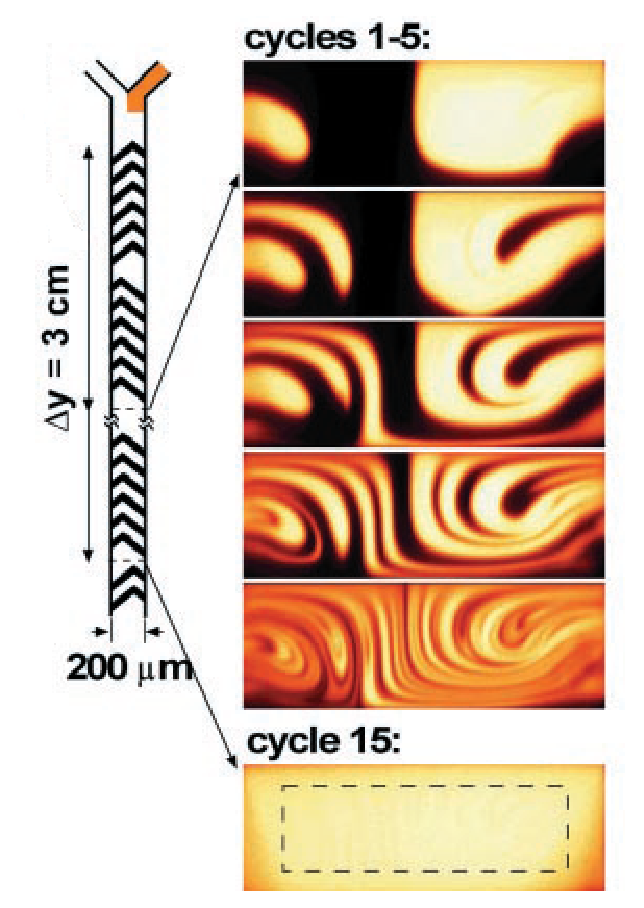
\includegraphics[width=0.21\textwidth]{stroockcrosssection}
     %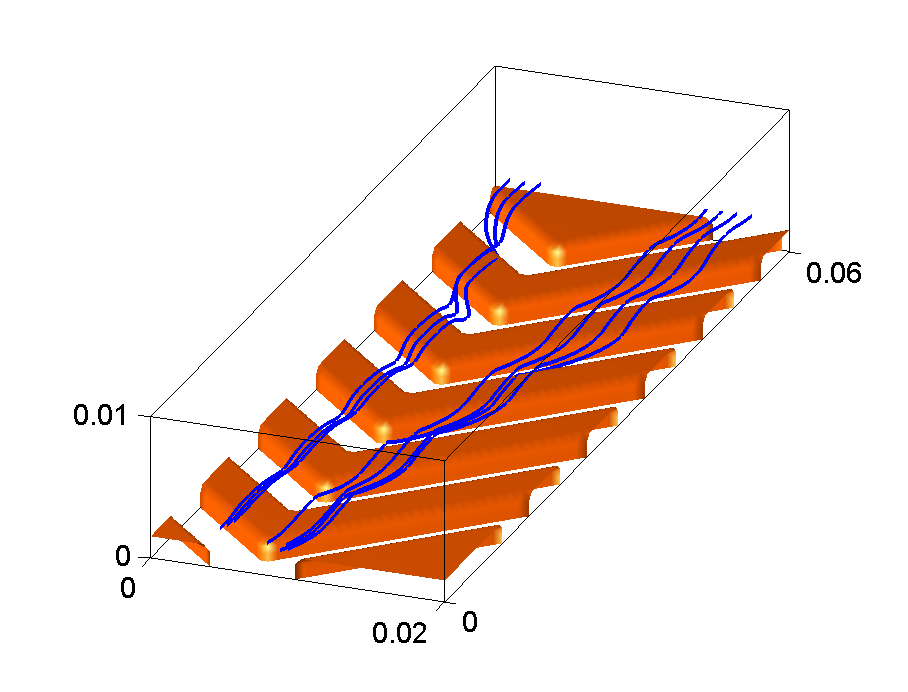
\includegraphics[width=0.35\textwidth]{stroockstructure}
     }
  \end{figure} 
  \vspace{-1cm}
  \begin{figure}
  \tiny{Stroock, Dertinger, Ajdari, Mezi\'c, Stone, Whitesides, \textit{Science} \textbf{295}(2002).} 
  \end{figure}
  \begin{itemize}
     \item Situation: low Re, high Pe.
     \item Goal: improve it by applying topology optimization on the half-cycle structure.
     \item Topology optimization rather than shape optimization. 
  \end{itemize}
\end{frame}

%%%%%%%%%%%%%%%%%%%%%%%%%%%%%%%%%%%%%%%%%%%%%%%%%%%%%%%%%%%%%%%%%%%%%%%
%%%%%%%%%%%%%%%%%%%%%%%%%%%%%%%%%%%%%%%%%%%%%%%%%%%%%%%%%%%%%%%%%%%%%%%
\begin{frame}
  \myframetitle{Topology Optimization of Microfluidic Channels}
%%%%%%%%%%%%%%%%%%%%%%%%%%%%%%%%%%%%%%%%%%%%%%%%%%%%%%%%%%%%%%%%%%%%%%% 

  \begin{itemize}
   \item Generalized Stokes equation for imcompressible flow (Darcey equation).
   \item Finite difference method with staggered mesh to solve the flow field ($180 \times 30 \times 60$ fluid/structure grid).
   \item A gradient-based optimization scheme with fixed step size.
   \item Adjoint method to find the gradient direction efficiently. 
   \item A Markov Chain model to approximate the solution of the advection-diffusion equation on the cross-sections of the channel.
   \item Fourth order Runge-Kutta method to integrate streamlines.
   \end{itemize}
   Tools
   \begin{itemize}
   \item PETSc (Portable, Extensible Toolkit for Scientific Computation).
   %\item Develope a package that communicates PETSc and Matlab
   \item 72-node cluster, 1GB RAM/CPU, gigabit ethernet.
   \end{itemize}
\end{frame}


%%%%%%%%%%%%%%%%%%%%%%%%%%%%%%%%%%%%%%%%%%%%%%%%%%%%%%%%%%%%%%%%%%%%%%%
%%%%%%%%%%%%%%%%%%%%%%%%%%%%%%%%%%%%%%%%%%%%%%%%%%%%%%%%%%%%%%%%%%%%%%%
%\begin{frame}
%\myframetitle{Without and With Diffusion}
%\begin{center}
%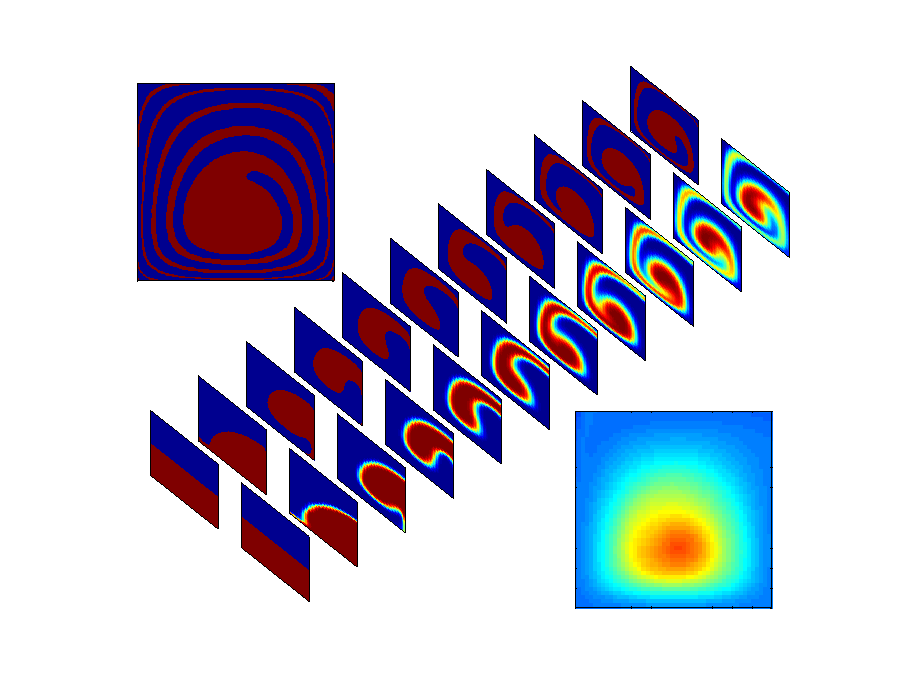
\includegraphics[width=0.83\textwidth,trim=0cm 1cm 0cm 0.5cm,clip]{markovvsexact}
%\end{center}
%\end{frame}


%%%%%%%%%%%%%%%%%%%%%%%%%%%%%%%%%%%%%%%%%%%%%%%%%%%%%%%%%%%%%%%%%%%%%%%
%%%%%%%%%%%%%%%%%%%%%%%%%%%%%%%%%%%%%%%%%%%%%%%%%%%%%%%%%%%%%%%%%%%%%%%
\begin{frame}
\myframetitle{Optimal $2$-D and $3$-D Structures}
  \begin{figure}
    \centerline{
    \begin{tabular}{cc}
      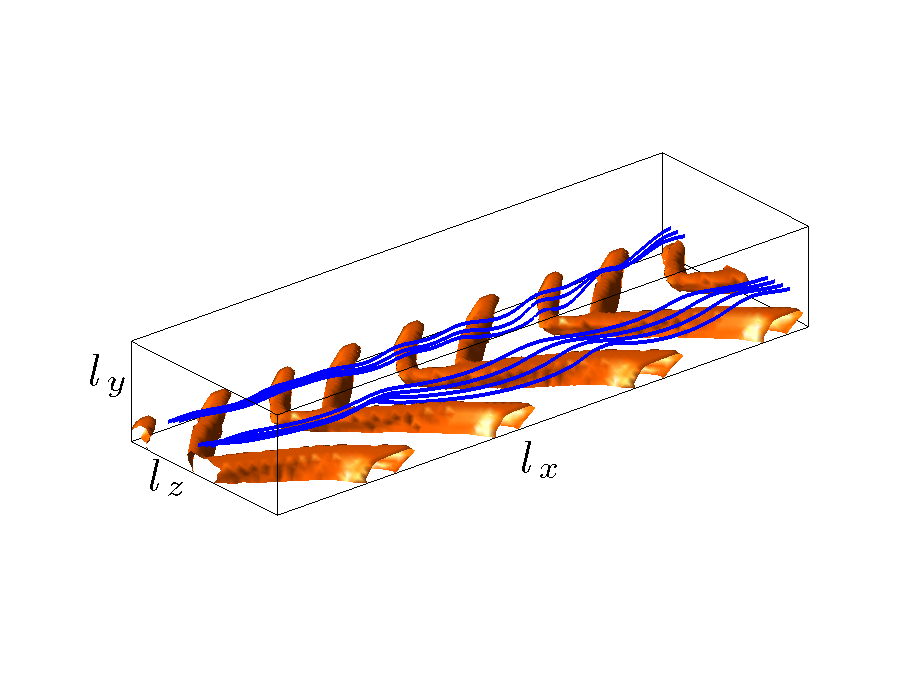
\includegraphics[width=0.4\textwidth,trim=1cm 0cm 1cm 1.6cm,clip]{example2structureherringbone}&
       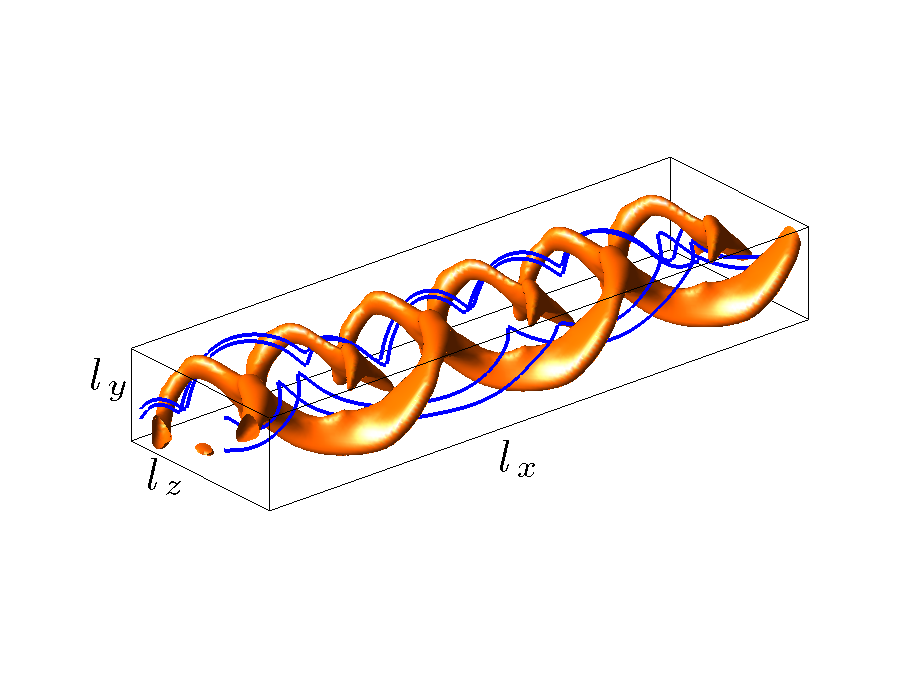
\includegraphics[width=0.4\textwidth,trim=1cm 0cm 1cm 1.6cm,clip]{example2structure3d}\\[-0.7cm]
      \footnotesize{Optimal herringbone channel} & \footnotesize{Optimal 3-D structured channel}
    \end{tabular} 
    }
  \end{figure}
%\vspace{-1cm}
  \begin{itemize}
    \item Improvement (in mixing length): 
        \begin{itemize}
        \item 30\% by optimal herringbone structure. 
        \item 60\% by optimal $3$-D structure.
        \end{itemize}
  \end{itemize}
\end{frame}


%%%%%%%%%%%%%%%%%%%%%%%%%%%%%%%%%%%%%%%%%%%%%%%%%%%%%%%%%%%%%%%%%%%%%%%%%
%%%%%%%%%%%%%%%%%%%%%%%%%%%%%%%%%%%%%%%%%%%%%%%%%%%%%%%%%%%%%%%%%%%%%%%%%
\begin{frame}
 \myframetitle{A Mixing Process Simulation}
    \begin{center}
      \includegraphics[width=0.6\textwidth]{chaoticmixing}
    \end{center}
  \begin{itemize}
    \item Simulated by a Markov Chain model and validated by comparing with experiments. 
  \end{itemize}
\end{frame}


%%%%%%%%%%%%%%%%%%%%%%%%%%%%%%%%%%%%%%%%%%%%%%%%%%%%%%%%%%%%%%%%%%%%%%%%
%%%%%%%%%%%%%%%%%%%%%%%%%%%%%%%%%%%%%%%%%%%%%%%%%%%%%%%%%%%%%%%%%%%%%%%%
\begin{frame}
  \myframetitle{Simulation of Standard Map with Small Diffusion}
%%%%%%%%%%%%%%%%%%%%%%%%%%%%%%%%%%%%%%%%%%%%%%%%%%%%%%%%%%%%%%%%%%%%%%% 

\centerline{
\includegraphics[width=0.75\textwidth,trim=1cm 1cm 0cm 0cm]{standardmapevolve}
}
   \begin{align*}
   \\[-1cm]
     \begin{cases}
        x_1 \leftarrow x_1+x_2 +\epsilon \sin{2 \pi x_1}  \mbox{ (mod } 1)\\
        x_2 \leftarrow  x_2 +\epsilon \sin{2 \pi x_1}     \mbox{ (mod } 1)
     \end{cases}
   \end{align*}
   \begin{equation*}
      \epsilon=0.3, \,\, f^0   = \cos(2\pi x_2)
   \end{equation*}

\end{frame}
%%%%%%%%%%%%%%%%%%%%%%%%%%%%%%%%%%%%%%%%%%%%%%%%%%%%%%%%%%%%%%%%%%%%%%%%
%%%%%%%%%%%%%%%%%%%%%%%%%%%%%%%%%%%%%%%%%%%%%%%%%%%%%%%%%%%%%%%%%%%%%%%%
\begin{frame}
  \myframetitle{Standard Map Cutoff}
%%%%%%%%%%%%%%%%%%%%%%%%%%%%%%%%%%%%%%%%%%%%%%%%%%%%%%%%%%%%%%%%%%%%%%% 

\begin{center}
    \includegraphics[width=0.45\textwidth,trim=1cm 1cm 0cm 0cm]{standardmapcutoff2}
  %  \includegraphics[width=0.45\textwidth,trim=1cm 1cm 0cm 0cm]{standardmapcutoffn2}
\end{center}
  \begin{itemize}
    \item The largest case is a Markov Chain with $6.4\times 10^9$ states.
    \item 51.2GB of memory is required to store a single state vector.
    \item The variance versus iteration trajectories present a cutoff. 
\end{itemize}

\end{frame}


%%%%%%%%%%%%%%%%%%%%%%%%%%%%%%%%%%%%%%%%%%%%%%%%%%%%%%%%%%%%%%%%%%%%%%%
%%%%%%%%%%%%%%%%%%%%%%%%%%%%%%%%%%%%%%%%%%%%%%%%%%%%%%%%%%%%%%%%%%%%%%%
\begin{frame}
  \myframetitle{Cutoff Phenomena in Chaotic Dynamics}
  \begin{itemize}
  \item Question: How many riffle shuffles to randomize $52$ cards?
    \begin{center}
      \includegraphics[width=0.55\textwidth,trim=1cm 1cm 0cm 0cm]{riffleshuffle}
    \end{center}
  \item Answer: 7.
  \item Aldous and Diaconis, 1986.
  \item A Markov Chain with $52! \approx 8 \times 10^{67}$ states.
  \end{itemize}
\end{frame}


%%%%%%%%%%%%%%%%%%%%%%%%%%%%%%%%%%%%%%%%%%%%%%%%%%%%%%%%%%%%%%%%%%%%%%%
%%%%%%%%%%%%%%%%%%%%%%%%%%%%%%%%%%%%%%%%%%%%%%%%%%%%%%%%%%%%%%%%%%%%%%%
\begin{frame}
 \myframetitle{Cutoff Phenomena in Chaotic Dynamics}
  \begin{itemize}
   \item A theoretical approach for the relation between cutoff phenomena in finite Markov Chains and chaotic mixing. 
   \item Generalize Symbolic Dynamics and create a new object called Stochastic Symbol Sequence to represent the evolution of a probability distribution by a chaotic map. 
   \item Successfully prove that the two things are coming from the same source.
   \item The process is composed of many (almost) independent processes $\Longrightarrow$ cutoff. 
  \end{itemize}
\end{frame}

%%%%%%%%%%%%%%%%%%%%%%%%%%%%%%%%%%%%%%%%%%%%%%%%%%%%%%%%%%%%%%%%%%%%%%%
\begin{frame}
 \myframetitle{Publications}
  \begin{itemize}
  \item Pratik Biswas, Tzu-Chen Liang, Kim-Chuan Toh, Ta-Chung Wang, and Yinyu Ye, “Semidefinite Programming Approaches for Sensor Network Localization with Noisy Distance Measurements”, IEEE Transactions on Automation Science and Engineering, vol. 3, issue 4, pp 360-371, Oct. 2006.
  \item Tzu-Chen Liang, Matthew West, “Topology Optimization of Microfluidic Mixing Channels”, in preparation, 2008.
  \item Tzu-Chen Liang, Matthew West, “Numerical Evidence of Cutoff Phenomena in Chaotic Mixing”, in preparation, 2008.
  \item Tzu-Chen Liang, Matthew West, “Cutoff Phenomena in Chaotic Dynamics”, in preparation, 2008.
  \end{itemize}
\end{frame}

\end{document}
